\section*{On UAMMD}

The \textbf{Universally Adaptable Multiscale Molecular Dynamics} project,
known as \textbf{UAMMD}, collects molecular simulation algorithms for Graphics 
Processing Units (GPUs) into header-only code. In layman's terms, this means 
that you can write programs in CUDA and include high-performance algorithms to 
carry out rigorous classical dynamics many-body simulations. UAMMD relies on the 
GPU's capacity to perform huge amounts of analogous computations in parallel to 
increase the speed at which it works out many-body interactions.

The program was written mostly by Ra\'ul P\'erez Pel\'aez as a PhD candidate at
UAM, in Madrid. As a consequence, it became strongly focused on the interests of
the author. If you would like to use UAMMD to carry out some particular type of
simulation like, say, ReaxFF molecular dynamics, then you will probably have to
code it yourself. However, he did implement some very advanced modules for
fluctuating hydrodynamics so, if your research lies on that path, you will
definitely want to check out UAMMD. In my view, the great strength of UAMMD
comes from the abstract methods it provides to deal with many-body interactions
on the GPU, allowing you to quickly write simple but extremely efficient
simulations.

%! codeblock: OnUAMMD
As the title of this book states, I aim to provide you with a painless 
introduction to writing UAMMD modules. I am writing with our research group's 
students in mind, imagining that you have begun to learn about molecular
simulation and have some (but not much) background in physics and programming.
If you need a more advanced approach, refer to the Wiki pages on the UAMMD
repository. Even if you don't, but you feel a painfully slow progress reading
this book, please skim through the pages and skip ahead until you find an
interesting section.
%! codeblockend

\section*{Beginner C++}

This section would be a good example of a chunk of text that you can skip and 
still be fine, as long as you have some very basic knowledge of what a C or C++ 
program looks like. The point here is \textit{not} to teach you C++, but rather 
to give you some basic feel for the language allowing you to read on and 
understand the gist of the code boxes. That should be enough for experimenting 
by tweaking the examples given here. You will, of course, eventually have to 
learn some CUDA if you wish to write advanced UAMMD programs, but there is a 
whole sea of free online resources out there. Instead of sailing out, it might 
be a good idea to understand what you want to know first (but if your desires 
draw you out to sea, by all means go forth and sail!).

Below, I have copied the iconic ``Hello, World'' program, written for C++. It
begins by including input/output functionality by adding the \texttt{iostream}
standard library to our program (\texttt{iostream} contains \texttt{cout} and
\texttt{endl} used a few lines down). We then specify that we will be using
the standard (\texttt{std}) versions of \texttt{cout} and \texttt{endl}, which
saves us from having to write \texttt{std::cout} or \texttt{std::endl} each
time we want to mention them.
\begin{lstlisting}
%! codefile: code/helloWorld.cpp
# include <iostream>

using std::cout;
using std::endl;

%! codeinsert: functionDefinitions
int main(int argc, char * argv[])
{
  cout<<"Hello, World!"<<endl;
  %! codeinsert: multiplesOfThree
  %! codeinsert: functionCalls
	return 0;
}
%! codeend
\end{lstlisting}

The final lines of code implement the \texttt{main} function. C++ programs
always execute this function first.

To define a function, we write the return value first, then the function name
followed by a list of arguments in parentheses. The contents come after the
arguments, so functions look like this:
\begin{lstlisting}
returnvalue functionname(list, of, arguments)
{
  what the function does
}
%!
\end{lstlisting}

Our ``Hello, World'' \texttt{main} function returns an integer (\texttt{int})
value: zero, in fact. As you can see, the function ends with \texttt{return 0;}.
Note that instructions end with a semicolon (;). The main function arguments, an
integer called \texttt{argc} and an array of strings called \texttt{argv}, refer
to the number of command-line arguments and the arguments themselves with which
the program was executed. In the next chapter, we will be passing these values
on to a UAMMD function that will deal with them. Here, we just ignore them.

The remaining line directs the ``\texttt{Hello, World!}'' string to standard
output, so that it would typically be printed on the screen, followed by an
end of line.

Compile the code above with \texttt{g++ helloWorld.cpp -o helloWorld}, or
something similar. Running the program should print ``Hello, World!'' on the
screen.

The compiler ignores anything you write between \texttt{/*} and \texttt{*/}, so
you can use these characters to insert explanatory comments in your code. In a
typicaly program, you will declare variables, data structures and classes, on
which you will later carry out some calculations. UAMMD code might include lines
like these.
\begin{lstlisting}
int numberOfParticles; /* An integer value */
real temperature; /* A floating-point real value */
Box simulationBox(10); /* A cubic box of side 10 units */
bool printPositions; /* A boolean (true or false) value */
%!
\end{lstlisting}

We will control program flow with \texttt{for} and \texttt{if}. A \texttt{for}
loop like
\begin{lstlisting}
  for(int i = 1; i <= 100; ++i) {
    cout<<"Iteration: "<<i<<endl;
  }
%!
\end{lstlisting}
will begin by setting the integer \texttt{i} equal to 1. It will then execute
the \texttt{cout} code on the line below time and again while \texttt{i} does
not exceed \texttt{100}. After each iteration of the code, it will increase the
variable \texttt{i} by one (this is what \texttt{++i} does). Each time, it
prints out ``\texttt{Iteration:}'', followed by the value of \texttt{i}.

When you want the program to do something different depending on whether 
something else happened, you typically write code with the following structure.
\begin{lstlisting}
  if(this_is_true) {
    then_do_this();
    and_this();
  }
%!
\end{lstlisting}
Sometimes you want to specify what the program should do otherwise by adding
\begin{lstlisting}
  else {
    do_this_instead();
  }
%!
\end{lstlisting}
For example, suppose we wanted to print the number only every thirteen steps,
then we would replace the content of the for loop like this.
\begin{lstlisting}
%! codeblock: multiplesOfThree
  int printEverynSteps = 13;

  for(int i = 1; i <= 100; ++i) {
    if(printEverynSteps > 0
       and i % printEverynSteps == 0) {
        cout<<"Iteration: "<<i<<endl;
    }
  }
%! codeblockend
\end{lstlisting}
The \texttt{if} block says that if \texttt{printEverynSteps} is a positive 
number (\texttt{> 0}) and the remainder of the step number divided by 
\texttt{printEverynSteps} equals zero (\texttt{step \% printEverynSteps == 0}), 
then the line is printed. Compiling and running the program outputs:
\begin{lstlisting}
Hello, World!
Iteration: 13
Iteration: 26
Iteration: 39
Iteration: 52
Iteration: 65
Iteration: 78
Iteration: 91
%!
\end{lstlisting}

Much of UAMMD code will be calling functions or methods defined elsewhere.
Let us add the following two functions before \texttt{main}.
\begin{lstlisting}
%! codeblock: functionDefinitions
int add(int a, int b) {
  return a + b;
}

void goodbye() {
  cout<<"Goodbye!"<<endl;
  return;
}
%! codeblockend
\end{lstlisting}
The first function takes two integers and returs their sum. The second takes no
arguments and returns none, but prints out ``Goodbye!''. To call these functions
after the \texttt{for} loop in our code, we simpy give their names followed by
their arguments in parentheses.
\begin{lstlisting}
%! codeblock: functionCalls
  cout<<"3 + 5 = "<<add(3,5)<<endl;
  goodbye();
%! codeblockend
\end{lstlisting}

\section*{\label{basic_simulation}Simulating classical particle physics}
\label{basic_simulation}

Numerical simulations of physical systems made up of particles usually involve
four steps.
\begin{enumerate}
  \item Declare the variables representing the state of the system.
  \item Set the variables to their initial values.
  \item Calculate how the system evolves in time by integrating the
        equations of motion, dealing with how each particle interacts with its
        environment.
  \item Print out final results and clean up.
\end{enumerate}

As an easy illustration, let us write a program for a bouncing rubber ball We 
begin by defining the simulation variables and parameters. Newton's second law 
tells us that the ball's acceleration $\mathbf{a}$ (which is the second 
derivative of the position $\mathbf{r}$ with respect to time) equals the 
acceleration of gravity.
\begin{equation*}
  \mathbf{a} = \frac{d^2\mathbf{r}}{dt^2} = \mathbf{g}.
\end{equation*}
Now, $\mathbf{g}$ equals $-9.8\ \mathrm{m/s}^2$ in the vertical direction. To
calculate the motion of the ball, we track the change in its position and
velocity in small increments of size \texttt{dt}. At every step, we change the
velocity by adding a change of $-9.8\ dt$ in the vertical direction and then
update the position by moving the ball to a new position using its current
velocity. Given $\mathbf{r}(n)$ and $\mathbf{v}(n)$, the position and velocity
at time step number $n$, we calculate the new position and velocity at time
$n + 1$ as
\begin{align*}
  \mathbf{r}(n + 1) & = \mathbf{r}(n) + \mathbf{v}(n)\ dt, \\
  \mathbf{v}(n + 1) & = \mathbf{v}(n) + \mathbf{g}\ dt.
\end{align*}
This simple numerical integration algorithm is known as the \textit{Euler
scheme}.

In our code, we will have to track the horizontal and vertical components of the 
position and velocity, which we store in the two-dimensional arrays \texttt{r} 
and \texttt{v}: \texttt{r[0]} will represent the horizontal coordinate and 
\texttt{r[1]} the vertical component, and similarly for \texttt{v[0]} and 
\texttt{v[1]}. Next, we will indicate the number of steps to calculate, the size 
of the time step and how often to print out the position.
\begin{lstlisting}
%! codefile: code/rubberBall.cpp
# include <iostream>

using std::cout;
using std::endl;

int main(int argc, char * argv[])
{
  /* State of the rubber ball */
  float r[2]; /* Position (measured in metres) */
  float v[2]; /* Velocity (in metres/second) */

  float g = -9.8; /* Acceleration of gravity (in m/s^2) */

  /* Integration parameters */
  int nsteps = 10000; /* Number of time steps to calculate */
  float dt = 0.001; /* Size of time step (in seconds) */
  int printEverynSteps = 20;
%! codepause
\end{lstlisting}
The second step on our list suggests that we specify the initial conditions.
\begin{lstlisting}
%! codecontinue: code/rubberBall.cpp
  /* Initial conditions */
  r[0] = 0;
  r[1] = 2;
  v[0] = 0.5;
  v[1] = 1;
%! codepause
\end{lstlisting}
Thirdly, we integrate the equations of motion with Euler's algorithm. When we
update the positions and velocities, we must take into account collisions with
the floor. If the ball hits the floor, the vertical component of its velocity
reverses and it looses some of its momentum. At the end of the \texttt{for}
loop we print out one in every 10 steps.
\begin{lstlisting}
%! codecontinue: code/rubberBall.cpp
  /* Euler integration of the equations of motion */
  for(int step = 0; step <= nsteps; ++step) {
    /* New position */
    r[0] = r[0] + v[0]*dt;
    r[1] = r[1] + v[1]*dt;

    /* New velocity */
    v[1] = v[1] + g*dt;

    /* Deal with collisions */
    if(r[1] <= 0 && v[1] < 0) {
      v[0] = 0.9*v[0];
      v[1] = -0.8*v[1];
    }

    /* Output state */
    if(printEverynSteps > 0
       && step % printEverynSteps == 0) {
      cout<<step*dt<<" "<<r[0]<<" "<<r[1]<<endl;
    }
  }
%! codeend
\end{lstlisting}
Finally, we close down the program.
\begin{lstlisting}
%! codecontinue: code/rubberBall.cpp
  cout<<"# Simulated time: "<<nsteps*dt<<" seconds. #"<<endl;
  return 0;
}
%! codeend
\end{lstlisting}
Compiling and running the code generated the data used to plot the trajectory
in Fig. \ref{rubberBall}.

\begin{figure}
  \centering
  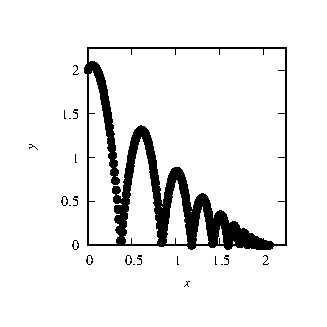
\includegraphics[width = 0.65 \textwidth]{figures/rubberBall.eps}
  \caption{\label{rubberBall}Trajectory of a bouncing rubber ball calculated
           with the code written in the previous pages.}
\end{figure}


\section*{Installing CUDA}

To make UAMMD programs, you will need to install a CUDA compiler and you will
have to run the programs on a compatible GPU device. Saying more would lead us
too far astray into a land that I do not wish to visit, so I recommend you check
the documentation for UAMMD and CUDA.

\begin{comment}
List of programs written in this chapter:

%! codeblock: codelist
* `helloWorld.cpp`: The iconic "Hello, World!" example written in C++.
* `rubberBall.cpp`: Simulation of a bouncing rubber ball.
%! codeblockend
\end{comment}
